\chapter{能量、曲率與輻射}

\lectureoverview{去掉兩項限制後，牛頓模型便能揭示更多物理意義。首先，共動星系的總能量不必恰為零；允許能量取任意值，便會引入 \(a^{-2}\) 項，而廣義相對論會將其重新詮釋為空間曲率。其次，宇宙中的物質來源不必是無壓物質。光子的波長會隨尺度因子伸長，因此輻射的密度會按 \(a^{-4}\) 稀釋，並使尺度因子遵循 \(a(t)\propto t^{1/2}\)。因此，同時含有物質與輻射的宇宙，在 \(a\) 較小時由輻射主導，在 \(a\) 較大時則由物質主導。在此過程中，我們將區分局部的牛頓運動與整體的相對論幾何，並指出哪些問題無法在沒有廣義相對論的情況下解決。}

\section{牛頓力學所能描述的}

在延伸模型之前，我們應先問：先前的牛頓計算為何能成立？物理宇宙由廣義相對論描述，其空間幾何未必在全域上是歐幾里得幾何。然而，任何光滑的彎曲空間，在足夠小的鄰域內都近似平坦。地球表面的一小塊看起來像平面；同樣地，遠小於曲率半徑的宇宙區域也可以視為平坦。

``小''是相對於曲率尺度而言。這個區域仍可能橫跨數十億光年。在其中，只要相鄰星系的相對特異速度是非相對論性的，且引力場微弱，就可以用牛頓力學描述它們。因此，牛頓計算並非與愛因斯坦理論競爭；它是更完整描述在局部、低速條件下的極限。

這裡有個立即浮現的警訊：輻射並非低速運動。光子以及仍處於相對論狀態的中微子，不能視為普通牛頓粒子組成的氣體。牛頓式推理仍可用來整理膨脹方程，但方程右側的源項必須從靜質量密度擴展為能量密度。這正是近似開始顯露其適用界限之處。

\section{回顧尺度因子}

取一個均勻分布的星系系統，並將座標附著在隨宇宙平均流動而移動的網格上。位於固定共動座標 \(x\) 的星系，與選定原點之間的物理距離為
\begin{equation}
D(t)=a(t)x
\label{eq:c02-distance}
\end{equation}
尺度因子 \(a(t)\) 將座標間距轉換為物理間距。

\(a\) 的絕對值是約定俗成的。若將所有共動座標乘上一個常數重新縮放，同一組物理距離也可以用 \(a\) 的反向縮放來表示。因此，\(a\) 和分配給單一座標格子的質量都不是各自不變的量。尺度因子的比值與分數膨脹率則是不變的：
\begin{equation}
\frac{a(t_2)}{a(t_1)},
\qquad
H(t)\equiv\frac{\dot a}{a}.
\label{eq:c02-hubble}
\end{equation}
事實上，若 \(a'=\alpha a\)，其中 \(\alpha\) 是固定常數，則 \(\dot a'/a'=\dot a/a\)。

令 \(\nu_m\) 表示每單位共動座標體積所含的質量。重新標記網格會改變它的數值；但在普通物質守恆時，它不隨時間改變。共動單位立方體的物理體積為 \(a^3\)，因此物質密度為
\begin{equation}
\boxed{\rho_m(a)=\frac{\nu_m}{a^3}.}
\label{eq:c02-matter-density}
\end{equation}
這種 \(a^{-3}\) 稀釋只是體積增大的結果：共動盒中的靜能保持不變，盒子的體積則持續增大。

真實的星系並非牢牢固定在網格上。它們會在星系群中繞行、落入星系團，並帶有相對於平均流動的小速度。尺度因子描述大尺度上的平滑運動；這些局部偏離稱為 \emph{特異速度}。

\begin{classroomqa}
\audiencequestion{每個星系都必須恰好沿徑向遠離其他每個星系嗎？}
\lecturerresponse{只有平均的哈伯流才呈現這種形式。星系的實際運動，是共同膨脹與附近結構所造成的特異速度之和。這就像河流的水流上疊加了漩渦：漩渦在局部很重要，卻不會抹去大尺度的流動。 \lecturetimestamp{00:24:47--00:26:33}}
\end{classroomqa}

對於總牛頓能量為零的無壓物質，前一講得到
\begin{equation}
H^2=\frac{8\pi G}{3}\rho_m
=\frac{8\pi G\nu_m}{3a^3}.
\label{eq:c02-zero-energy-friedmann}
\end{equation}
由於整體網格的歸一化方式可以任意選擇，我們暫且選取單位，使 \(8\pi G\nu_m/3=1\)。在膨脹分支上，
\begin{equation}
\frac{\dot a}{a}=\frac{1}{a^{3/2}},
\qquad
\dot a=\frac{1}{\sqrt a}.
\end{equation}
將導數取倒數並積分，得到
\begin{equation}
\frac{dt}{da}=\sqrt a,
\qquad
t-t_B=\frac{2}{3}a^{3/2},
\end{equation}
其中 \(t_B\) 是這個理想化解達到 \(a=0\) 的時刻。因此
\begin{equation}
\boxed{a(t)\propto (t-t_B)^{2/3}.}
\label{eq:c02-matter-law}
\end{equation}
在這個僅含物質的臨界模型中，宇宙會永遠膨脹。由於 \(\dot a\propto a^{-1/2}\)，膨脹速率會減慢；但 \(\dot a\) 不會在任何有限的 \(a\) 值處降為零。

\begin{figure}[ht]
\centering
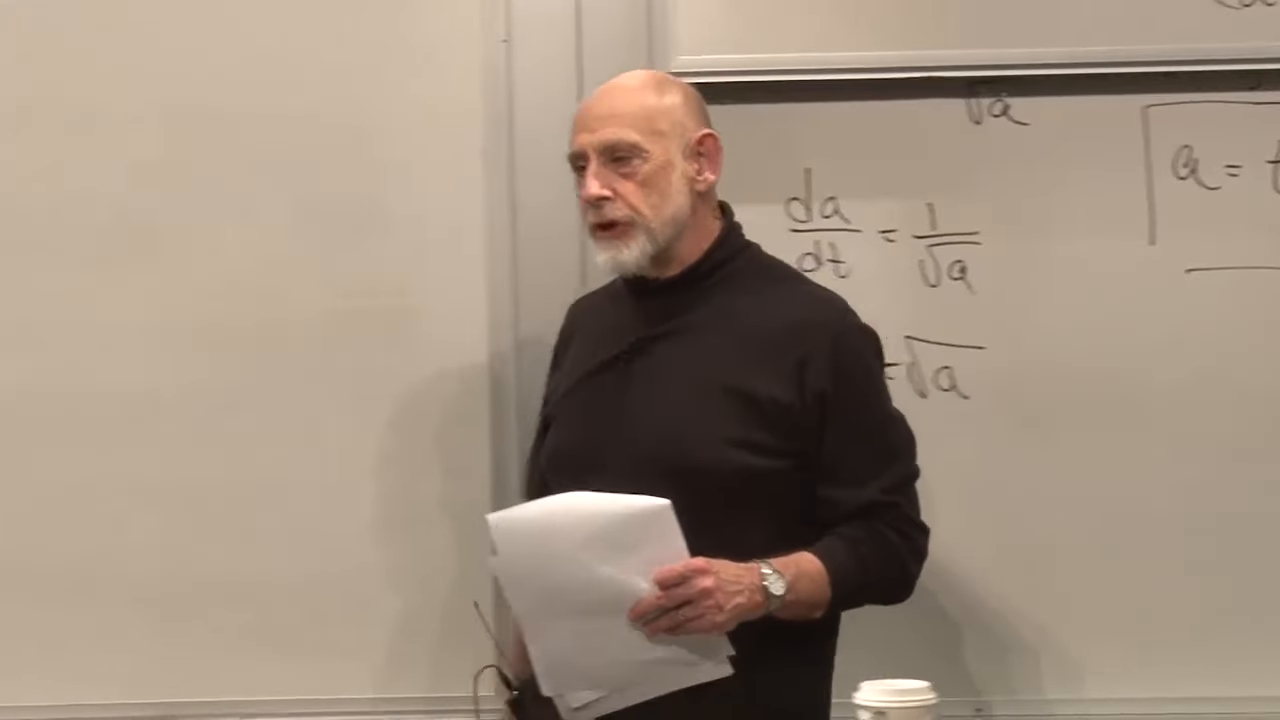
\includegraphics[width=0.68\textwidth]{lecture_02_figure_02.png}
\caption{複習板記下了 \(\dot a=1/\sqrt a\)，以及框出的物質主導膨脹定律 \(a\propto t^{2/3}\)。中間的代數推導有部分被遮住，內容由方程式~\eqref{eq:c02-zero-energy-friedmann}--\eqref{eq:c02-matter-law}補上。}
\label{fig:c02-matter-recap}
\lectureframe{00:29:20.838}
\end{figure}

\begin{classroomqa}
\audiencequestion{為什麼捨棄負的平方根？}
\lecturerresponse{方程式本身並沒有捨棄它。方程式~\eqref{eq:c02-zero-energy-friedmann}決定的是 \(H^2\)，而非 \(H\) 的正負號。正根描述膨脹，負根描述收縮。行星引力場中的岩石可以向外或向內運動，卻都遵守同一個能量方程式；選擇哪個分支取決於初始條件。我們選擇膨脹分支，因為討論的宇宙正處於膨脹狀態。 \lecturetimestamp{00:23:09--00:24:46}}
\end{classroomqa}

下一個模型仍會忽略暗能量。這是刻意的安排：先理解較早期的物質與輻射框架，再加入主導當前加速膨脹時期的成分。相較之下，暗物質已包含在物質項中，因為非相對論性暗物質也按 \(a^{-3}\) 稀釋。

\begin{classroomqa}
\audiencequestion{暗能量難道不是今天的主導成分嗎？}
\lecturerresponse{是的。這裡介紹的雙成分圖像，是當前加速膨脹被發現之前的標準教學宇宙學。暗物質歸入物質；暗能量則是將另行引入的第三種成分。從較早期的模型開始，能讓我們看清每增加一個項會帶來什麼改變。 \lecturetimestamp{00:28:02--00:28:45}}
\end{classroomqa}

\section{恢復能量常數}

零能量只是特殊的初始條件。為了不再限制能量為零，回到均勻球體邊界上一個質量為 \(m\) 的星系。令其共動半徑為 \(x\)，則
\begin{equation}
D=ax,
\qquad
\dot D=\dot a x.
\label{eq:c02-comoving-particle}
\end{equation}
牛頓殼層定理指出，只有球體內的質量 \(M(D)\) 會影響徑向加速度；外部球殼不會施加淨力。該星系守恆的牛頓能量為
\begin{equation}
\frac{1}{2}m\dot D^{\,2}-\frac{GM(D)m}{D}=E.
\label{eq:c02-newton-energy}
\end{equation}
兩個項中都應包含因子 \(m\)。在黑板上快速書寫時很容易漏掉它，但保留這個因子，便能看清最後的常數表示每單位受測質量的能量。

均勻性讓我們可以把代表性星系選在 \(x=1\)。於是 \(D=a\)、\(\dot D=\dot a\)，而球體的
\begin{equation}
V_{\rm sph}=\frac{4\pi}{3}a^3,
\qquad
M(a)=\rho_m V_{\rm sph}=\frac{4\pi}{3}\rho_m a^3.
\label{eq:c02-enclosed-mass}
\end{equation}
黑板上用 \(V\) 表示體積，也在旁註中用它表示徑向速度。我們改用不會混淆的符號 \(V_{\rm sph}\) 和 \(\dot D\)。

\begin{figure}[ht]
\centering
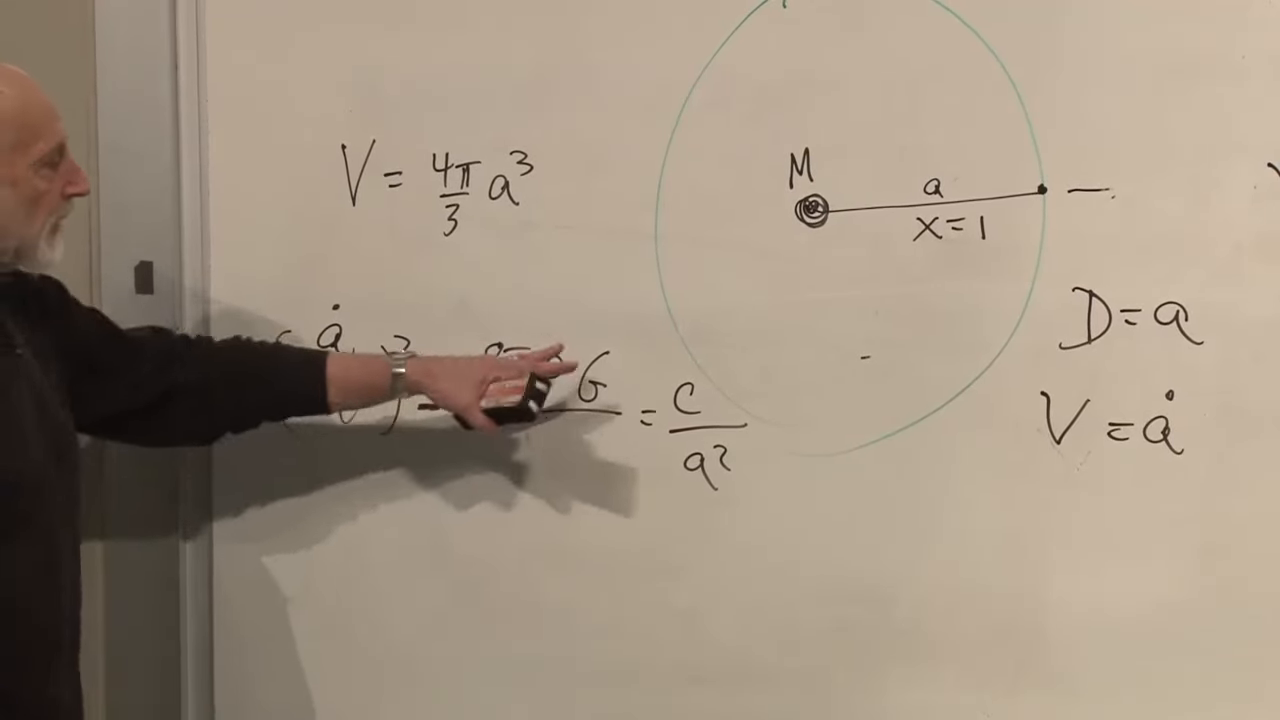
\includegraphics[width=0.86\textwidth]{lecture_02_figure_03.png}
\caption{包住質量的球體與非零能量的弗里德曼方程式。圖中可見的標記包括 \(V_{\rm sph}=4\pi a^3/3\)、中心質量 \(M\)、\(x=1\)、\(D=a\) 和 \(\dot D=\dot a\)。講者遮住了部分方程式，以下將以代數推導重建。}
\label{fig:c02-energy-board}
\lectureframe{00:37:59.876}
\end{figure}

\begin{figure}[ht]
\centering
\begin{tikzpicture}[scale=1.05,>=Latex]
  \draw[thick] (0,0) circle (2.6);
  \fill (0,0) circle (2.2pt) node[below left=2pt] {\(M(a)\)};
  \draw[thick,->] (0,0) -- (2.58,0);
  \fill (2.6,0) circle (2.2pt) node[right=4pt] {galaxy \(m\)};
  \node[above] at (1.30,0.04) {\(D=ax\)};
  \node[below] at (1.30,-0.04) {\(x=1\Rightarrow D=a\)};
  \draw[->,blue!60!black,thick] (2.63,0.18) -- (3.55,0.72)
    node[right] {\(\dot D=\dot a\)};
  \node at (0,-3.05) {\(M(a)=\frac{4\pi}{3}\rho_m a^3\)};
\end{tikzpicture}
\caption{在 \(x=1\) 處的牛頓球體示意圖，經清楚重繪如下。外部球殼的作用互相抵消，因此邊界星系只受內部包圍質量的影響。}
\label{fig:c02-sphere-redraw}
\end{figure}

將 \(D=a\) 代入方程式~\eqref{eq:c02-newton-energy}，除以 \(m/2\)，並定義常數
\begin{equation}
C\equiv\frac{2E}{m}.
\end{equation}
可得
\begin{equation}
\dot a^{\,2}-\frac{2GM(a)}{a}=C.
\label{eq:c02-energy-a}
\end{equation}
再除以 \(a^2\)，並利用方程式~\eqref{eq:c02-enclosed-mass}，得到
\begin{equation}
\left(\frac{\dot a}{a}\right)^2-
\frac{8\pi G}{3}\rho_m=\frac{C}{a^2},
\label{eq:c02-energy-form}
\end{equation}
等價地，
\begin{equation}
\boxed{H^2=\frac{8\pi G}{3}\rho_m+\frac{C}{a^2}.}
\label{eq:c02-friedmann-C}
\end{equation}
這就是以牛頓能量約定表示的無壓物質第一弗里德曼方程式。新的 \(a^{-2}\) 項記錄了代表性星系的初始能量高於、等於或低於逃逸能量。

代入 \(\rho_m=\nu_m/a^3\) 後，令
\begin{equation}
A_m\equiv\frac{8\pi G\nu_m}{3}>0,
\end{equation}
於是
\begin{equation}
H^2=\frac{A_m}{a^3}+\frac{C}{a^2},
\qquad
\dot a^{\,2}=\frac{A_m}{a}+C.
\label{eq:c02-energy-branches}
\end{equation}
與其立即積分，不如先從不同極限來看這個方程式，會更能看出其中的物理意義。

\subsection{正能量}

若 \(C>0\)，則在 \(a\) 很小時，物質項 \(A_m/a^3\) 佔主導。因此，早期膨脹仍遵循物質主導定律 \(a\propto t^{2/3}\)。但在 \(a\) 很大時，\(C/a^2\) 項會在 \(H^2\) 中佔主導，亦即
\begin{equation}
\dot a^{\,2}\longrightarrow C.
\end{equation}
膨脹速率會趨近常數，
\begin{equation}
a(t)\sim\sqrt C\,t.
\label{eq:c02-positive-late}
\end{equation}
這相當於宇宙學中的情形：把蘋果以高於逃逸速度的速度拋出。引力持續使它減速，但到了遠處，蘋果仍保有非零的漸近速度。

\subsection{零能量}

當 \(C=0\) 時，方程式~\eqref{eq:c02-energy-branches}回到臨界解 \(a\propto t^{2/3}\)。宇宙會無限膨脹，而 \(\dot a\) 趨近於零。這正是能量恰好等於逃逸能量的情形。

\subsection{負能量}

若 \(C=-|C|<0\)，則
\begin{equation}
H^2=\frac{A_m}{a^3}-\frac{|C|}{a^2}
=\frac{A_m-|C|a}{a^3}.
\label{eq:c02-negative-energy}
\end{equation}
尺度因子不能大於
\begin{equation}
a_{\max}=\frac{A_m}{|C|},
\label{eq:c02-amax}
\end{equation}
因為右側在此處降為零。膨脹分支到達 \(a_{\max}\) 時，\(\dot a=0\)；之後解便接續到收縮分支。用牛頓圖像來說，這就像以低於逃逸速度拋出蘋果：它先上升，接著轉向落下。

\begin{classroomqa}
\audiencequestion{右側等於 \(H^2\)，因此不能為負；模型又怎麼會重新坍縮？}
\lecturerresponse{它從未變成負值。膨脹期間，右側逐漸減小，並在 \(a_{\max}\) 處降為零。此時 \(H=0\)。接著，解從正平方根轉換為負平方根，並以 \(\dot a<0\) 沿允許範圍折返。若讓該表示式越過零繼續延伸，看似合理，實則錯誤。它不能越過零：零是邊界，而不是實數 \(H\) 可以穿越的值。 \lecturetimestamp{00:48:43--00:53:03}}
\end{classroomqa}

因此，三種牛頓能量對應三種不同的定性演化史：\(C<0\) 時重新坍縮，\(C=0\) 時達到臨界逃逸，而 \(C>0\) 時則永遠膨脹，且 \(\dot a\) 漸近趨於常數。接下來令人意外的是，廣義相對論會為這些相同情形賦予幾何意義。

\section{從能量到曲率}

將方程式~\eqref{eq:c02-friedmann-C}中的能量項移到幾何一側，並定義
\begin{equation}
k\equiv-C.
\label{eq:c02-k-definition}
\end{equation}
於是
\begin{equation}
\boxed{H^2+\frac{k}{a^2}=\frac{8\pi G}{3}\rho.}
\label{eq:c02-friedmann-k}
\end{equation}
黑板上的記號在 \(C\)、\(K\) 和 \(\kappa\) 之間交替；將該項移過等號時，也吸收了一個負號。方程式~\eqref{eq:c02-k-definition}確立了此處採用的約定：正牛頓能量對應 \(k<0\)，零能量對應 \(k=0\)，負牛頓能量對應 \(k>0\)。

\begin{figure}[ht]
\centering
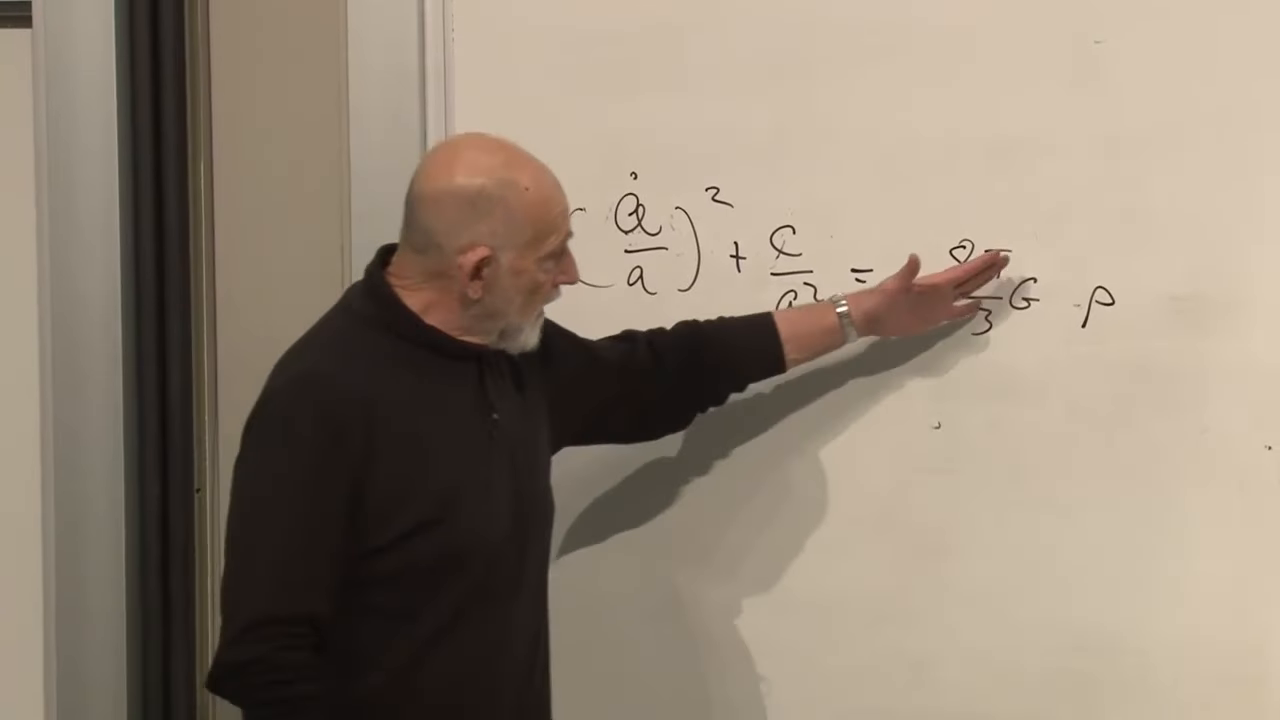
\includegraphics[width=0.76\textwidth]{lecture_02_figure_04.png}
\caption{將弗里德曼方程式整理成左側為幾何、右側為源項。這個畫面呈現了兩者的概念區分；它並未展示完整的張量形式愛因斯坦方程式。}
\label{fig:c02-geometry-source}
\lectureframe{00:55:22.810}
\end{figure}

這種排列是愛因斯坦方程式的簡化版本。左側描述幾何：\(H\) 描述膨脹，\(k/a^2\) 描述空間曲率。右側描述物質源。在牛頓力學中，源項是質量密度；在相對論中，源項是能量與動量，完整地由應力能量張量表示。對均勻且各向同性的宇宙，第一弗里德曼方程式取決於總能量密度 \(\rho\)。

若保留一般單位，質量密度會透過靜止能量 \(\rho_{\rm mass}c^2\) 貢獻於方程式。從此處開始，我們設定 \(c=1\)，因此質量與能量使用相同單位。此時符號 \(\rho\) 可以包含靜止質量、動能、輻射，以及任何其他均勻的能量成分。

\begin{figure}[ht]
\centering
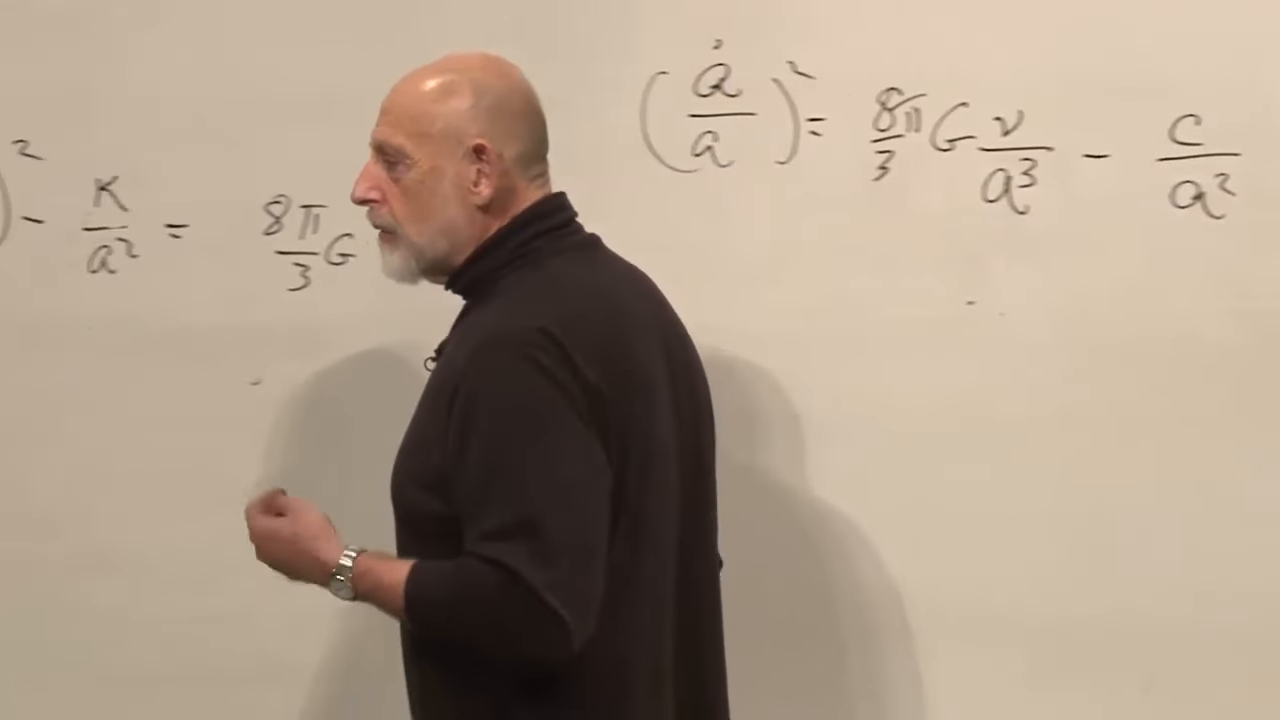
\includegraphics[width=0.88\textwidth]{lecture_02_figure_05.png}
\caption{黑板上並列的兩種弗里德曼方程式形式：以 \(\rho\) 表示的曲率形式，以及代入 \(\rho_m=\nu_m/a^3\) 後得到的物質形式。黑板上的記號有所變化；此處的符號約定則由方程式~\eqref{eq:c02-k-definition}固定。}
\label{fig:c02-curvature-comparison}
\lectureframe{00:57:52.659}
\end{figure}

幾何詮釋涉及全域結構。在相對論模型中，\(k=0\) 描述平坦的空間切片，\(k>0\) 描述正曲率的球面切片，\(k<0\) 描述負曲率的雙曲切片。牛頓推導在沒有這些全域幾何的情況下，重現了相同的演化方程式。因此，非零能量常數雖極其精確地模擬了曲率，卻不是推導出彎曲空間本身。

\begin{classroomqa}
\audiencequestion{既然牛頓力學與廣義相對論的幾何不同，為什麼兩者會得到相同的膨脹方程式？}
\lecturerresponse{廣義相對論也包含平坦的情形，而且任何光滑幾何在局部都近似平坦。更令人驚訝的是，牛頓能量常數在演化方程式中的位置，恰好就是相對論空間曲率所占的位置。兩者的動力學公式一致，但全域詮釋不同：歐幾里得的牛頓空間並沒有暗中變成球面或雙曲空間。這三種幾何必須在廣義相對論中建構。 \lecturetimestamp{01:20:59--01:24:20}}
\end{classroomqa}

\section{膨脹盒中的輻射}

現在來改變宇宙的內容物。考慮一個共動單位立方體，其物理體積為 \(a^3\)。對非相對論性物質而言，盒中的粒子數固定，每個粒子的靜止能量也近似固定，因此 \(\rho_m\propto a^{-3}\)。輻射則還有另一種效應：宇宙膨脹時，每個光子的能量都會降低。

波長為 \(\lambda\) 的光子，其能量為
\begin{equation}
E_\gamma=\frac{hc}{\lambda},
\qquad
E_\gamma\propto\lambda^{-1}.
\label{eq:c02-photon-energy}
\end{equation}
在均勻膨脹下，自由傳播的波長會隨尺度因子拉長：
\begin{equation}
\frac{\lambda(t_2)}{\lambda(t_1)}
=\frac{a(t_2)}{a(t_1)},
\qquad
\lambda\propto a.
\label{eq:c02-redshift}
\end{equation}
這就是宇宙學紅移，意味著
\begin{equation}
E_\gamma\propto a^{-1}.
\label{eq:c02-photon-redshift}
\end{equation}
若共動盒中的光子數守恆，其輻射總能量會按 \(a^{-1}\) 降低。再除以物理體積 \(a^3\)，得到
\begin{equation}
\boxed{\rho_r(a)=\frac{\nu_r}{a^4}.}
\label{eq:c02-radiation-density}
\end{equation}
此處 \(\nu_r\) 是自由傳播輻射密度的常數振幅。輻射密度比物質密度多出一個 \(a\) 的反比次方：三次方來自空間稀釋，另一次方則來自每個光子的紅移。

吉他弦的類比有助於建立直覺。弦上的一個振動模態包含整數個半波長。若緩慢拉長弦，這個整數不可能連續改變；波長會隨弦長調整。同樣地，緩慢膨脹的環上的波，其節點數是絕熱不變量，因此波長會隨環的周長改變。一般的波都可以分解成這類模態。

這不能取代在膨脹時空中求解麥克斯威方程組；它只是方程式~\eqref{eq:c02-redshift}背後有依據的直覺：幾何緩慢膨脹時，物理波長會改變，而模態標記保持不變。

\begin{classroomqa}
\audiencequestion{這個論證需要導電或反射的盒子嗎？在沒有實體邊界的空曠膨脹空間中會怎樣？}
\lecturerresponse{盒壁只是記帳工具，並非聲稱宇宙被導體包圍。完整的證明來自膨脹度規中的波傳播。此處的論證採用一項經觀測且由相對論推導出的事實：自由傳播的波長會隨 \(a\) 改變。盒子有助於計算光子數與物理體積，但不會造成宇宙學紅移。 \lecturetimestamp{01:02:21--01:04:37}}
\end{classroomqa}

\begin{classroomqa}
\audiencequestion{波長為什麼會跟著網格改變，而不是保持固定的物理長度？}
\lecturerresponse{考慮一個環上的模態，其周長絕熱地改變。整數節點數不能連續漂移，因此允許的波長必須隨環的周長改變。將一般波展開為傅立葉模態，也會逐一得到相同結論。這提供了所需的絕熱直覺；精確的敘述則屬於彎曲時空中的場論。 \lecturetimestamp{01:34:18--01:38:33}}
\end{classroomqa}

\subsection{輻射主導的解}

暫且忽略曲率，將方程式~\eqref{eq:c02-radiation-density}代入弗里德曼方程式：
\begin{equation}
H^2=\frac{8\pi G\nu_r}{3a^4}
\equiv\frac{A_r}{a^4},
\qquad A_r>0.
\label{eq:c02-radiation-friedmann}
\end{equation}
在膨脹分支上，
\begin{equation}
\frac{\dot a}{a}=\frac{\sqrt{A_r}}{a^2},
\qquad
\dot a=\frac{\sqrt{A_r}}{a}.
\end{equation}
因此
\begin{equation}
a\,da=\sqrt{A_r}\,dt,
\qquad
\frac{a^2}{2}=\sqrt{A_r}(t-t_B),
\end{equation}
並且
\begin{equation}
\boxed{a(t)\propto(t-t_B)^{1/2}.}
\label{eq:c02-radiation-law}
\end{equation}
指數 \(1/2\) 和 \(2/3\) 的差異看似不大，物理意義卻至關重要。早期宇宙的膨脹率、溫度、反應凍結時刻與視界大小，都取決於哪種成分佔主導。

\section{物質與輻射組成的宇宙}

對於各自守恆的物質與輻射，總密度是兩者密度之和：
\begin{equation}
\rho(a)=\rho_m(a)+\rho_r(a).
\end{equation}
為了比較，先忽略曲率：
\begin{equation}
\boxed{H^2=\frac{C_m}{a^3}+\frac{C_r}{a^4},}
\label{eq:c02-mixed-friedmann}
\end{equation}
其中 \(C_m,C_r>0\)。黑板一開始將兩個係數標為 \(C_1\) 與 \(C\)；講者隨後口頭更正第二個符號，指出它是另一個常數。方程式~\eqref{eq:c02-mixed-friedmann}清楚呈現了這項更正。

\begin{figure}[ht]
\centering
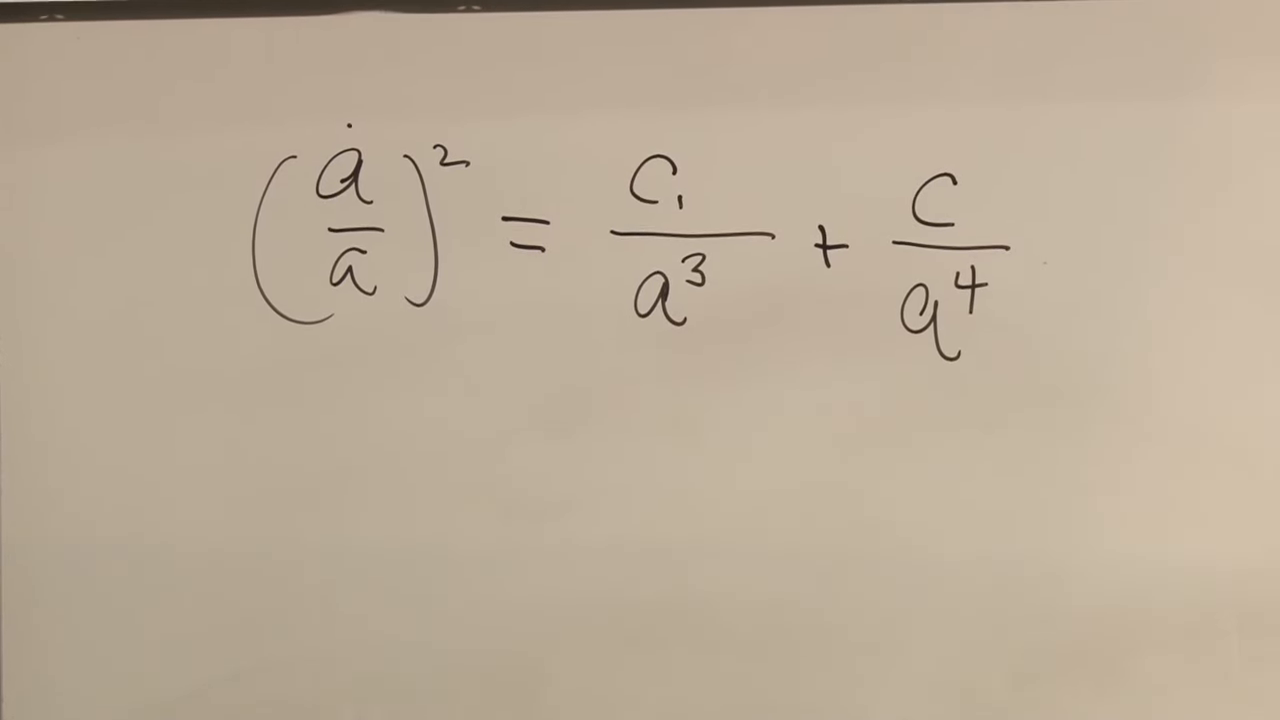
\includegraphics[width=0.74\textwidth]{lecture_02_figure_06.png}
\caption{黑板上的物質與輻射混合方程式。寫下的第二個係數後來被更正為輻射專屬常數，在方程式~\eqref{eq:c02-mixed-friedmann}中記為 \(C_r\)。}
\label{fig:c02-mixed-board}
\lectureframe{01:11:37.997}
\end{figure}

當 \(a\) 很小時，輻射項較大，因為 \(a^{-4}\) 比 \(a^{-3}\) 增長得更快：
\begin{equation}
a\ll a_{\rm eq}
\quad\Longrightarrow\quad
H^2\simeq\frac{C_r}{a^4},
\qquad
a(t)\propto t^{1/2}.
\end{equation}
當 \(a\) 較大時，則由物質項佔優：
\begin{equation}
a\gg a_{\rm eq}
\quad\Longrightarrow\quad
H^2\simeq\frac{C_m}{a^3},
\qquad
a(t)\propto t^{2/3}.
\end{equation}
令兩項相等，即可直接求得相等時的尺度：
\begin{equation}
a_{\rm eq}=\frac{C_r}{C_m}.
\label{eq:c02-equality-scale}
\end{equation}
物質輻射相等與光子退耦並非同一事件。前者問的是兩種能量密度何時相等；後者問的是交互作用何時不再使物質與輻射維持熱平衡。

輻射成分包含光子，以及任何以超相對論速度運動的粒子。極輕的中微子在足夠高的溫度下也有這種行為；引力子背景的密度也會以相同方式變化。帶質量的粒子一旦變為非相對論性，其主要的靜止質量貢獻便開始像物質一樣變化。冷暗物質屬於 \(C_m/a^3\)，而非輻射項。

\begin{classroomqa}
\classquestion{方程式~\eqref{eq:c02-mixed-friedmann}中，哪一項先佔主導，之後又是哪一項佔主導？}
\lecturerresponse{當 \(a\) 很小時，\(a^{-4}\) 的增長快於 \(a^{-3}\)，因此早期膨脹由輻射主導，並遵循 \(a\propto t^{1/2}\)。隨著 \(a\) 增大，輻射與物質之比按 \(1/a\) 降低；之後膨脹改由物質主導，遵循 \(a\propto t^{2/3}\)。 \lecturetimestamp{01:11:46--01:13:38}}
\end{classroomqa}

\begin{classroomqa}
\audiencequestion{物質與輻射的相對含量是否假設為常數？}
\lecturerresponse{密度並非常數，但在各成分停止有效交換能量，且粒子的生成或湮滅可以忽略之後，係數 \(C_m\) 和 \(C_r\) 可以視為常數。此時，物質的共動靜止質量守恆，自由輻射的共動光子數也守恆；紅移則使輻射多出一個 \(a^{-1}\) 因子。在交互作用劇烈或粒子種類發生湮滅的時期，這套記帳方式需要進一步修正。 \lecturetimestamp{01:13:39--01:14:53}}
\end{classroomqa}

\begin{classroomqa}
\audiencequestion{物質與輻射何時停止強烈交互作用？}
\lecturerresponse{粗略估計，光子在 \(10^5\) 年左右與普通物質退耦。精確的復合歷程留待後續計算，且不應與物質--輻射相等混淆。此處只需知道，退耦之後，這兩種成分大致可以分開追蹤。 \lecturetimestamp{01:27:29--01:27:46}}
\end{classroomqa}

\begin{classroomqa}
\audiencequestion{在還沒有星系可用來追蹤膨脹之前，我們怎麼知道早期曾有過 \(a\propto t^{1/2}\) 時期？}
\lecturerresponse{我們根據膨脹留下的物理紀錄推知其歷史。原初核合成取決於早期反應速率與 \(H(t)\) 之間的競爭；宇宙微波背景則記錄了較晚期的熱狀態與擾動。星系觀測讓物質時期的行為較容易直接研究，而輻射時期則是根據這些早期宇宙的證據重建。 \lecturetimestamp{01:27:46--01:30:10}}
\end{classroomqa}

物質加輻射模型刻意保留了不完整性。它是描述宇宙從輻射主導轉變為物質主導的經典框架。當前的加速膨脹需要另一種源，即暗能量；它會帶來性質迥異的新項。

\section{紅移後的能量去了哪裡}

\(E_\gamma\propto a^{-1}\)的降低引出一個無法迴避的問題：光子的能量去了哪裡？若想像一個帶有反射壁的盒子隨宇宙膨脹，輻射會施加壓力並對盒壁做功。熱力學關係為
\begin{equation}
dE=-p\,dV.
\label{eq:c02-pdv}
\end{equation}
隨著 \(V\) 增大，輻射能量減少。損失的能量可能轉化為盒壁運動物體的動能、應變能或熱。

共動盒沒有實體盒壁。它是隨平均膨脹移動的假想邊界。光子會穿越這個邊界；但在均勻的輻射背景中，統計上流入的通量與流出的通量相抵。即使它不是容器，仍可作為記帳體積。壓力做功定律依然描述共動體積內能量的演化。

對輻射而言，\(p=\rho/3\)，而 \(E=\rho V\)。方程式~\eqref{eq:c02-pdv}於是給出
\begin{align}
d(\rho V)&=-\frac{\rho}{3}\,dV,\\
V\,d\rho&=-\frac{4}{3}\rho\,dV,\\
\frac{d\rho}{\rho}&=-\frac{4}{3}\frac{dV}{V}.
\end{align}
由於 \(V\propto a^3\)，積分後得到 \(\rho\propto a^{-4}\)，與波長的論證一致。這項熱力學推導也清楚表明，減少的不只是數密度，每個光子的能量也會降低。

\begin{classroomqa}
\audiencequestion{紅移後的光子能量去了哪裡？宇宙總能量守恆嗎？}
\lecturerresponse{若有實體盒壁，輻射會對壁做功，因此能量轉移可用一般的力學帳目描述。但對整個宇宙而言，問題更為微妙。全域能量守恆通常源自時間平移對稱性；膨脹時空一般不具時間平移不變性，因此未必有唯一且守恆的總能量。雖然可以建立有用的牛頓類比，來討論膨脹的能量，但要對全域情形作出確定的陳述，仍需要廣義相對論。這裡兩種描述都有用，但牛頓模型無法導出最終的全域結論。 \lecturetimestamp{01:16:51--01:20:58}}
\end{classroomqa}

\begin{classroomqa}
\audiencequestion{如果共動盒是想像出來的，光子又會穿越邊界，壓力做功的圖像為什麼仍然有用？}
\lecturerresponse{均勻性補足了所需的記帳方式。平均而言，每個離開某個共動體積的光子，都會由鄰近體積進入的光子在統計上補足。局部通量平均後彼此抵消，但物理體積與波長仍會改變。反射盒讓做功機制更具體；共動盒則在沒有實體壁的情況下，呈現相同的平均守恆定律。 \lecturetimestamp{01:24:22--01:27:28}}
\end{classroomqa}

\begin{classroomqa}
\audiencequestion{膨脹只會降低光子密度，還是也會降低每個光子的能量？}
\lecturerresponse{兩者都會發生。每單位物理體積中的光子數按 \(a^{-3}\) 降低，而宇宙學紅移又使每個光子的能量多降低一個 \(a^{-1}\) 因子。這相當於輻射的絕熱冷卻。普通氣體在緩慢膨脹並做功時也會冷卻，不過突然的自由膨脹是另一種熱力學過程。 \lecturetimestamp{01:42:30--01:45:55}}
\end{classroomqa}

\section{退行、視界與模型的極限}

哈伯定律將退行速率
\begin{equation}
v_{\rm rec}=HD
\label{eq:c02-recession}
\end{equation}
賦予在選定宇宙時間切片上、距離為 \(D\) 的物體。當 \(D\) 足夠大時，方程式~\eqref{eq:c02-recession}可能給出大於 \(c\) 的值。這不違反狹義相對論，因為 \(v_{\rm rec}\) 並非在單一局部慣性參考系中測得的鄰近物體速度；它比較的是變化幾何中相距遙遠的共動世界線。每位局部觀測者測得的光速仍是 \(c\)，而且沒有任何局部物質物體會以超光速超越另一個物體。

\begin{classroomqa}
\audiencequestion{足夠遙遠的星系會以超光速退行嗎？}
\lecturerresponse{會，其宇宙學退行速率 \(HD\)可以超過 \(c\)。但沒有任何局部物體會以超光速超越鄰近的觀測者，這個結果也不能用來超光速傳遞訊號。這裡描述的是遙遠共動世界線之間固有距離的變化，而不是在單一事件處測得的普通狹義相對論速度。\lecturetimestamp{01:30:17--01:32:13}}
\end{classroomqa}

超光速退行本身無法判定現在發出的光最終是否會到達我們。這取決於未來整段膨脹歷史。在減速的物質主導模型中，目前退行速度超過光速的區域，之後仍可能變得可觀測，因為相關視界會隨時間演化。如果加速膨脹持續下去，事件視界可能使足夠遙遠的事件永遠無法被觀測到。

\begin{classroomqa}
\audiencequestion{星系的退行速率一旦超過光速，就會消失嗎？}
\lecturerresponse{事情沒有這麼簡單。穿越哈勃半徑和真正的事件視界是兩種不同的概念。在減速模型中，來自目前退行速度超過光速之區域的光，之後仍可能到達我們。若暗能量持續主導宇宙演化，整體因果結構就會改變，並可能形成最終視界。要判定哪些訊號會抵達，必須知道時空幾何，不能只看 \(HD\) 的某一瞬間快照。\lecturetimestamp{01:32:14--01:34:18}}
\end{classroomqa}

將狹義相對論的說法應用於全域時，也可能造成誤解。粒子的不變靜止質量不會隨速度增加；它的能量和動量則取決於觀測者所在的局部參考系。有質量粒子無法被加速至超過局部光速，但遙遠共動星系的退行，並不是它穿越單一局部參考系的過程。

\begin{classroomqa}
\audiencequestion{快速退行的星系會有較大的相對論質量嗎？}
\lecturerresponse{最好避免使用``相對論質量''這個說法。星系具有不變的靜止質量，而它的能量和動量則與參考系有關。此外，跨越宇宙學距離所定義的退行速率，並不是狹義相對論公式中的局部速度。只有透過時空度規比較遙遠事件，這些概念才會相符。\lecturetimestamp{01:38:34--01:40:05}}
\end{classroomqa}

\begin{classroomqa}
\audiencequestion{遙遠星系的退行速率超過光速時，時間軸和空間軸會如何變化？}
\lecturerresponse{不存在一個單一的全域洛侖茲參考系，可以藉由其傾斜的座標軸解決這個問題。狹義相對論比較平直時空中的慣性參考系；宇宙學則需要一個度規，描述如何在延展的彎曲時空中連結各個局部參考系。牛頓式推理在小範圍內仍然可靠，但要建立全域描述，就得等到廣義相對論。\lecturetimestamp{01:40:07--01:42:30}}
\end{classroomqa}

牛頓能量守恆導出了物質的正確尺度因子方程，甚至預見了曲率項。波動力學和熱力學則提供了輻射的標度關係。然而，空間幾何、全域能量和視界都不是局部的牛頓問題；它們需要以下將介紹的度規描述。

\section{物質、輻射與曲率}

僅含物質的臨界解滿足
\begin{equation}
\rho_m\propto a^{-3},
\qquad
a(t)\propto t^{2/3}.
\end{equation}
還原牛頓能量（以單位質量計）後，得到
\begin{equation}
H^2=\frac{8\pi G}{3}\rho_m+\frac{C}{a^2}.
\end{equation}
\(C\)為正時，宇宙會永遠膨脹，且晚期有 \(a\sim t\)；\(C=0\)時為臨界逃逸；\(C\)為負時，尺度因子會達到最大值，之後宇宙再坍縮。定義 \(k=-C\)，便可將同一項放在相對論弗里德曼方程的幾何側。

輻射與物質不同，因為宇宙膨脹既會改變數密度，也會改變每個量子的能量：
\begin{equation}
\begin{aligned}
\lambda&\propto a,
&\qquad E_\gamma&\propto a^{-1},\\
\rho_r&\propto a^{-4},
& a(t)&\propto t^{1/2}.
\end{aligned}
\end{equation}
因此，雙組分方程
\begin{equation}
H^2=\frac{C_m}{a^3}+\frac{C_r}{a^4}
\end{equation}
描述的宇宙早期由輻射主導，之後進入物質主導時期。暗能量、空間幾何，以及視界的因果結構都不在這個模型的範圍內；這些正是牛頓近似告訴我們必須交由廣義相對論處理的問題。